\section{Implementation and Performance Assessment}\label{sec:exp}

\begin{figure}[]
\centering
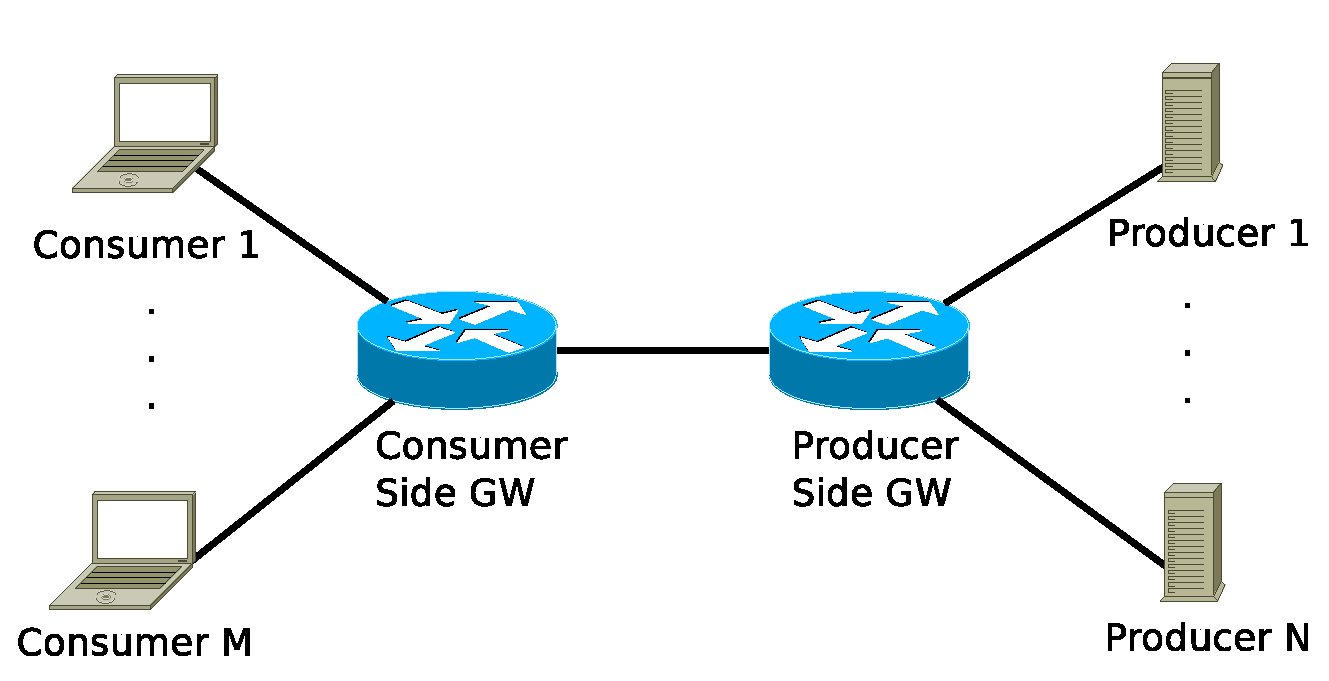
\includegraphics[width=\columnwidth]{images/testnet.eps}
\caption{Testbed network topology. $M$ consumers and $N$ producers}\label{testnet}
\end{figure}

\begin{figure}[]
\centering
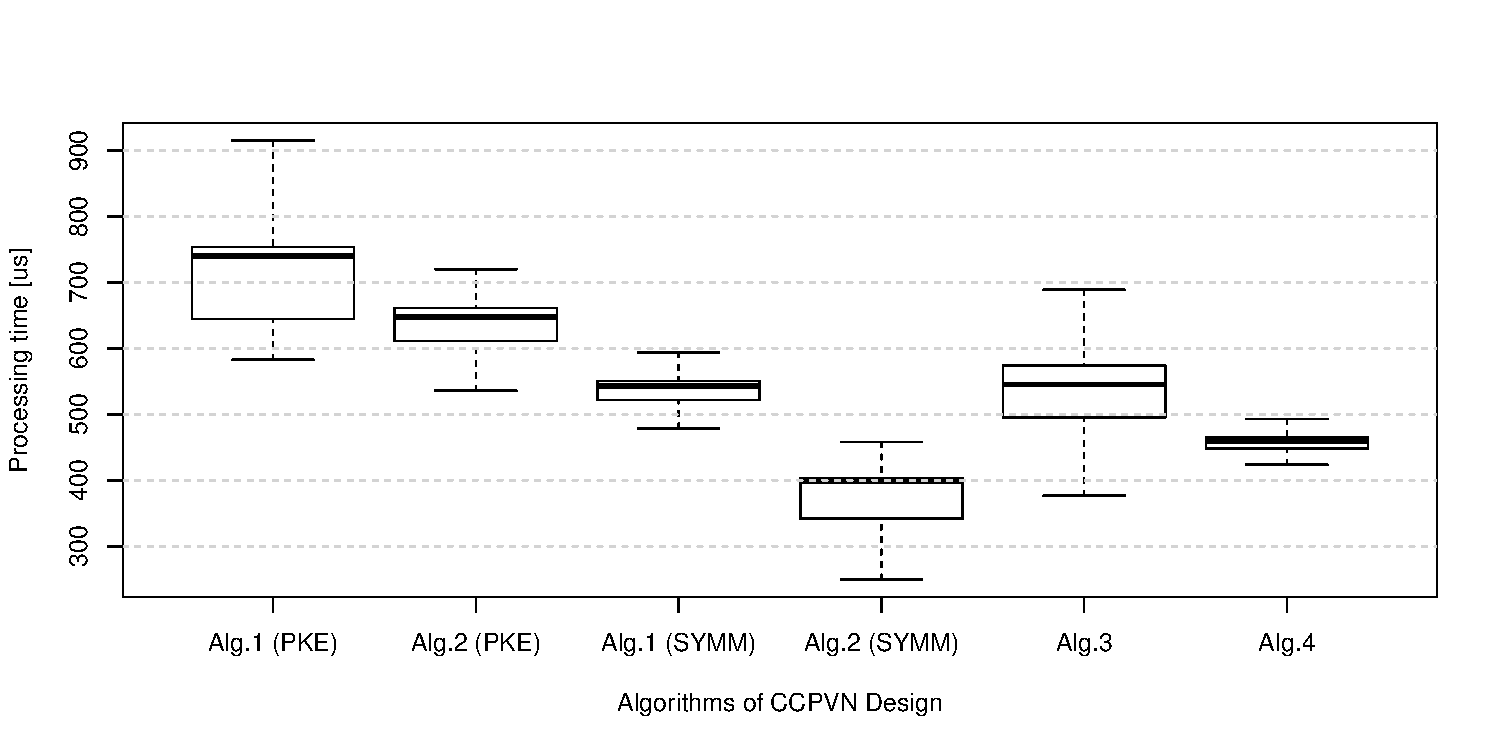
\includegraphics[width=\columnwidth]{images/times.pdf}
\caption{Execution time of the algorithms in CCVPN design}\label{times}
\end{figure}

\begin{figure}[]
\centering
  \subfigure[Throughput]{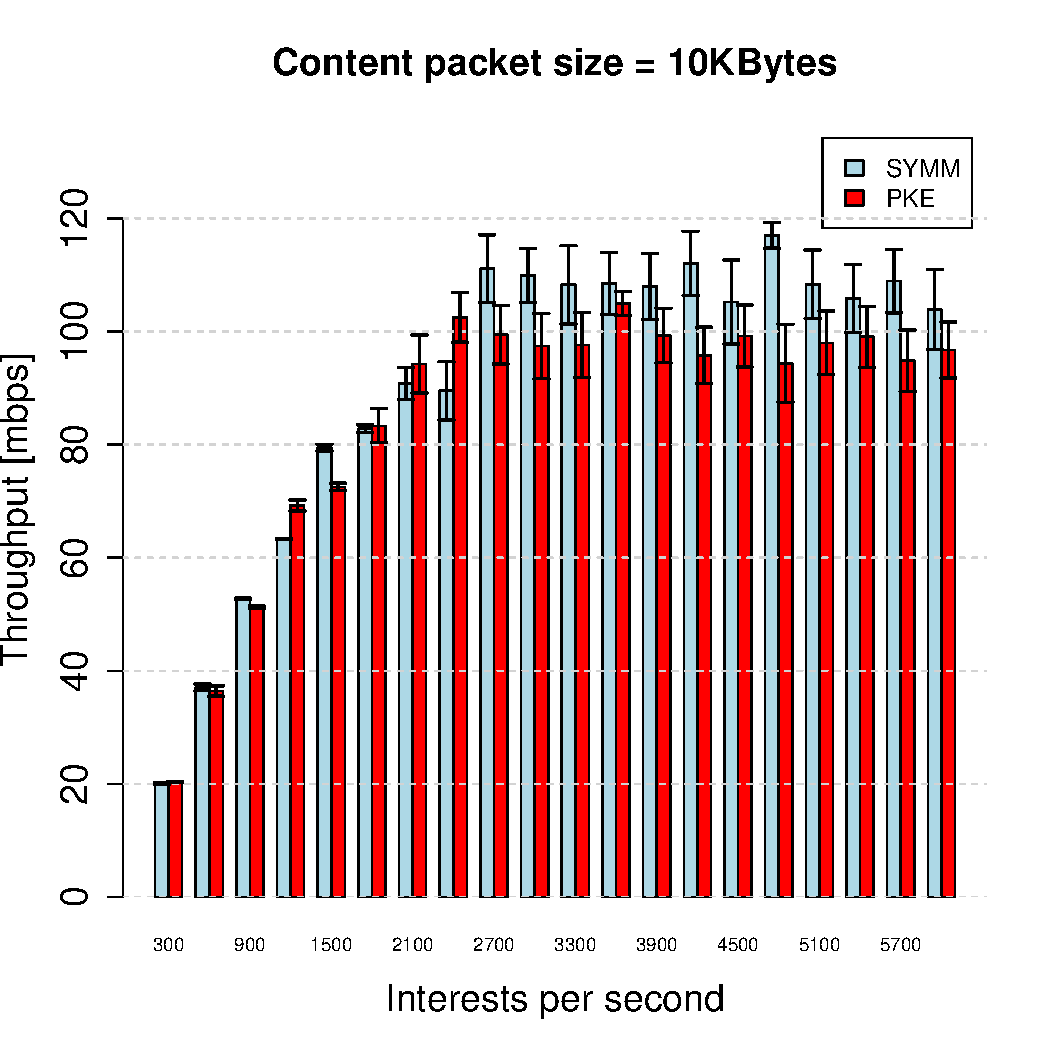
\includegraphics[width=0.8\columnwidth]{images/1_1_thput.pdf}\label{1a}}
  \hfil
  \subfigure[Avg. RTT]{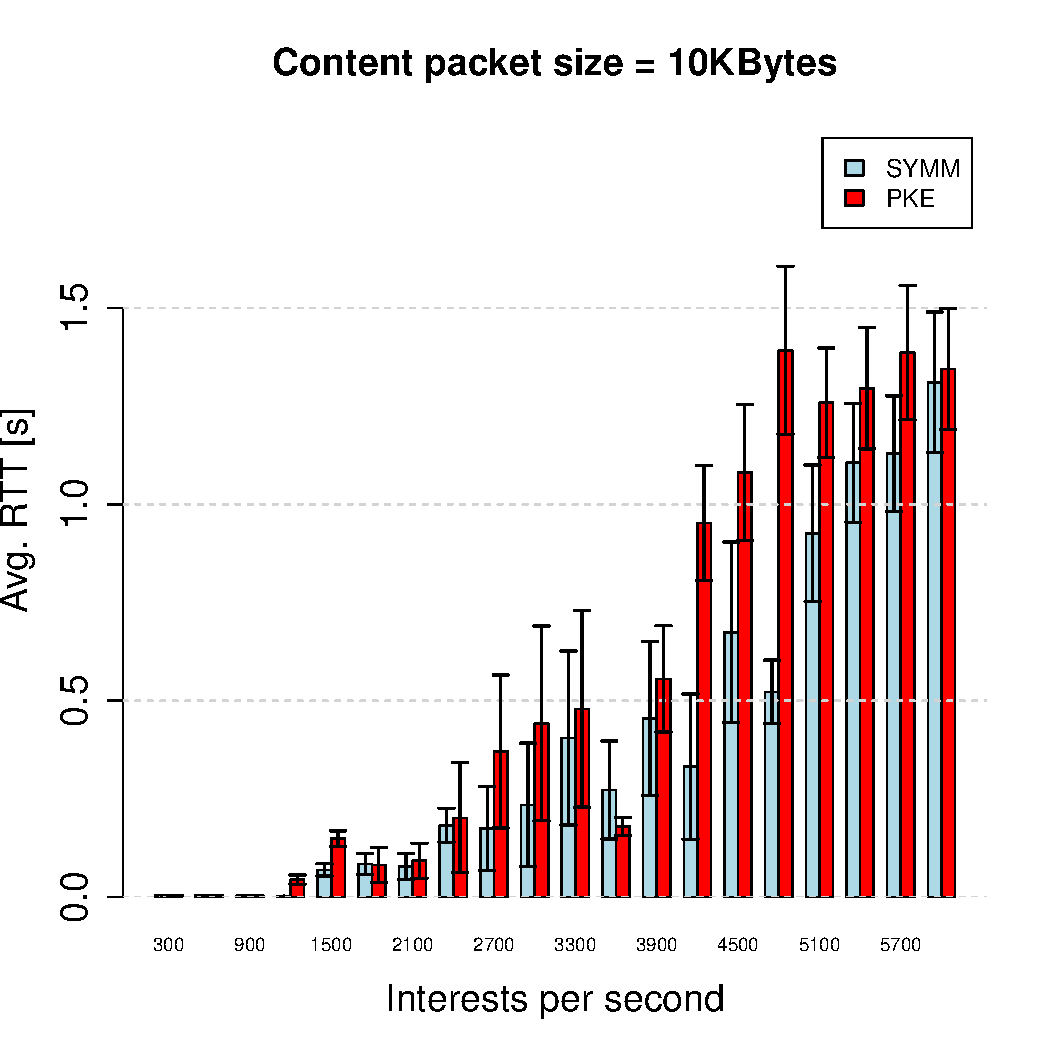
\includegraphics[width=0.8\columnwidth]{images/1_1_rtt.pdf}\label{1b}}
\caption{CCVPN performance with one consumer and one producer for increasing interest issuance rates.}\label{exp1}
\end{figure}

\begin{figure}[]
\centering
  \subfigure[Throughput]{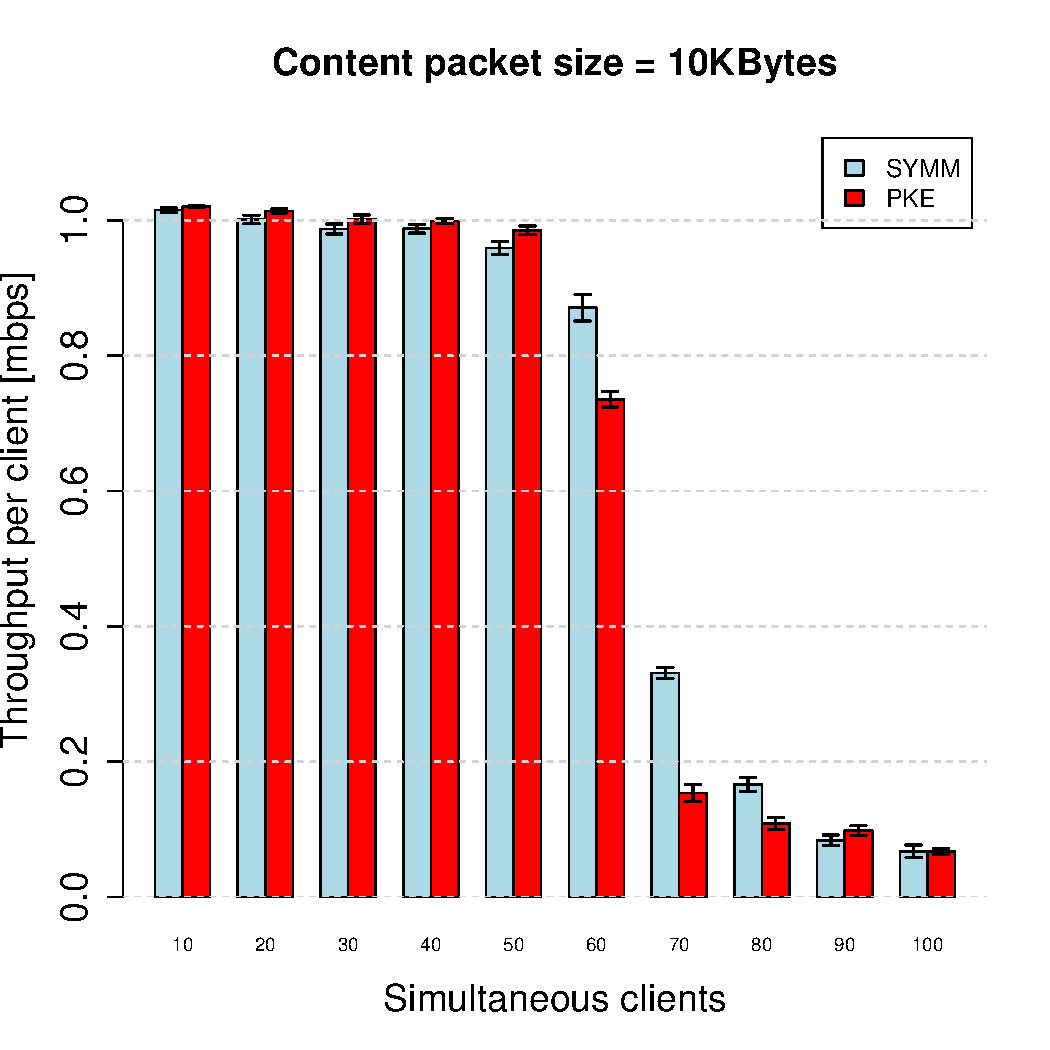
\includegraphics[width=0.8\columnwidth]{images/n_1_thput.pdf}\label{1a}}
  \hfil
  \subfigure[Avg. RTT]{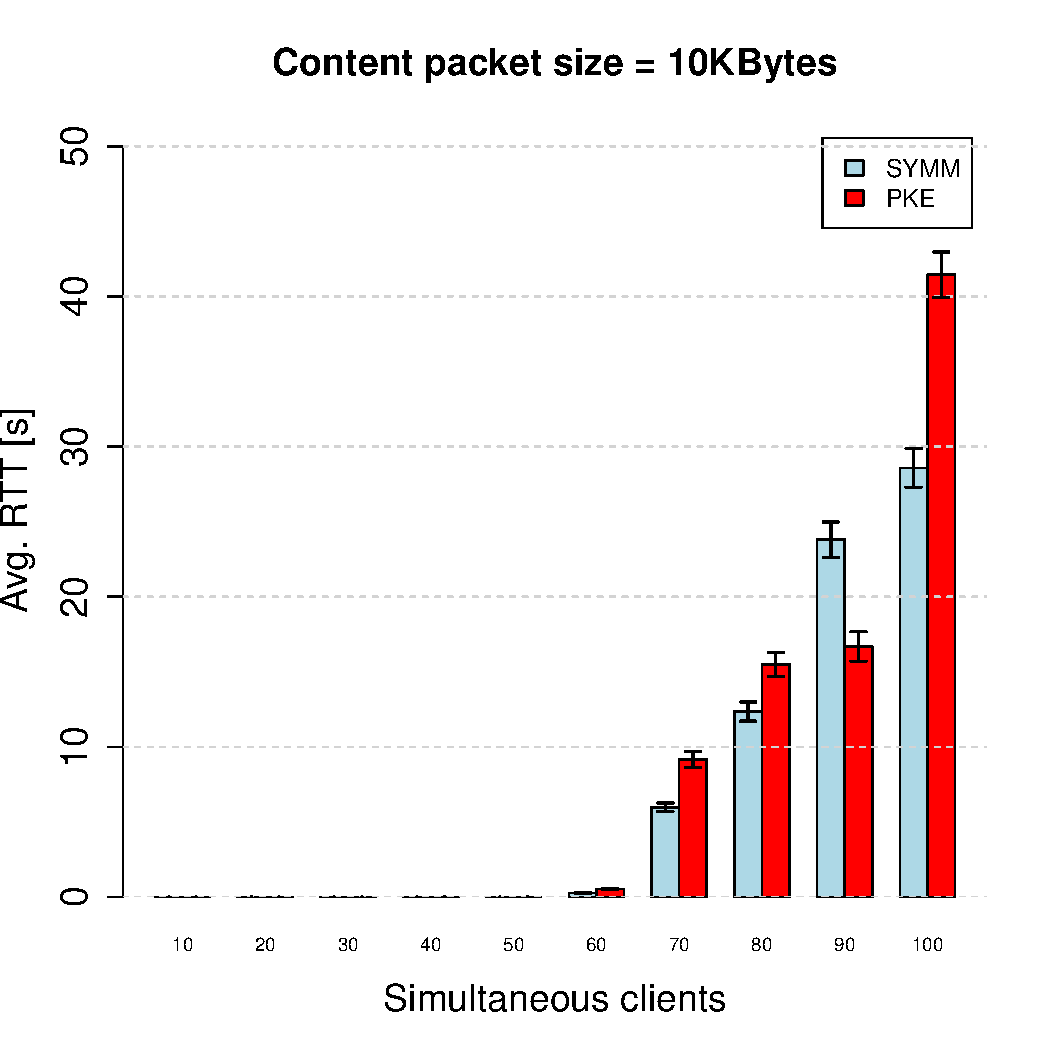
\includegraphics[width=0.8\columnwidth]{images/n_1_rtt.pdf}\label{1b}}
\caption{CCVPN performance with multiple consumers and one producer. Each consumer requests with 1 mbps rate.}\label{exp1}
\end{figure}

\begin{figure}[]
\centering
  \subfigure[Throughput]{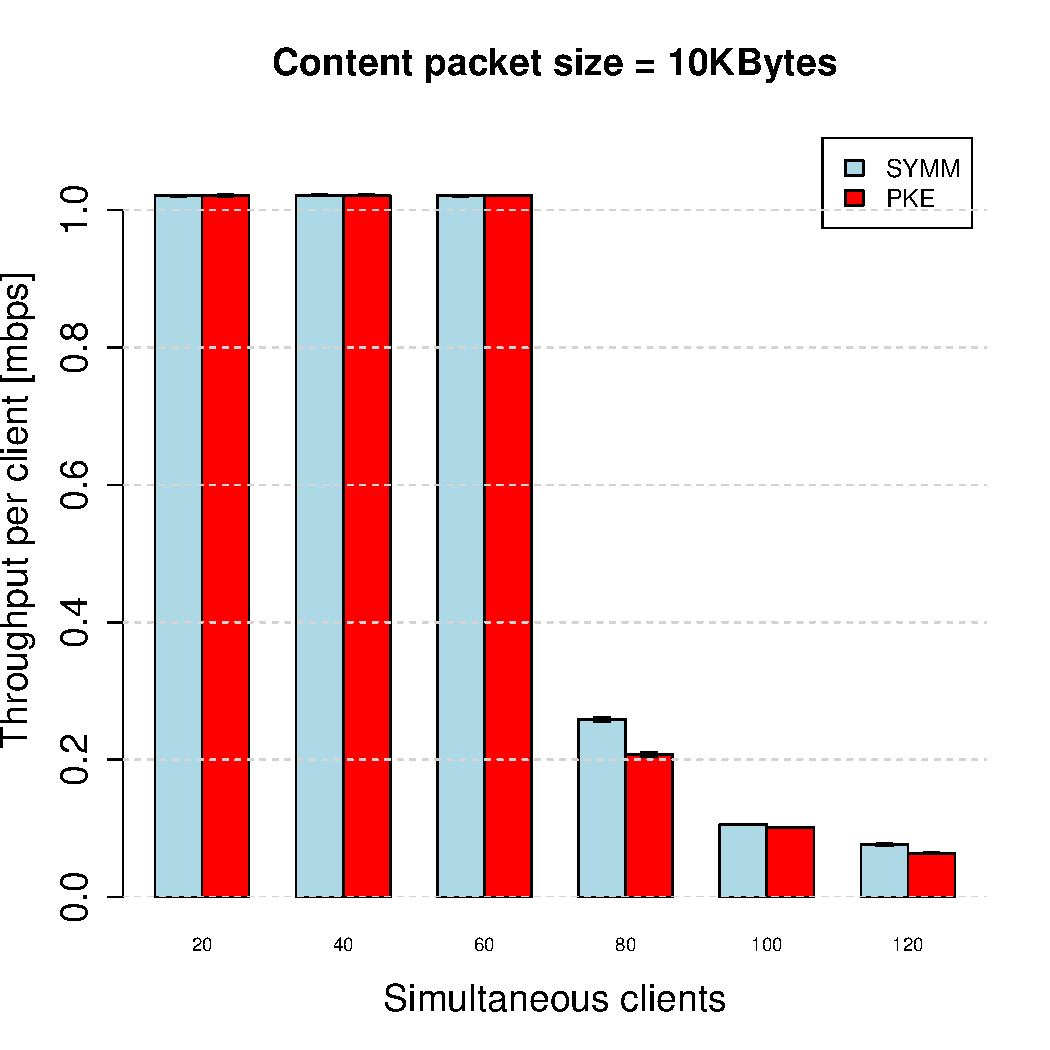
\includegraphics[width=0.8\columnwidth]{images/n_n_thput.pdf}\label{1a}}
  \hfil
  \subfigure[Avg. RTT]{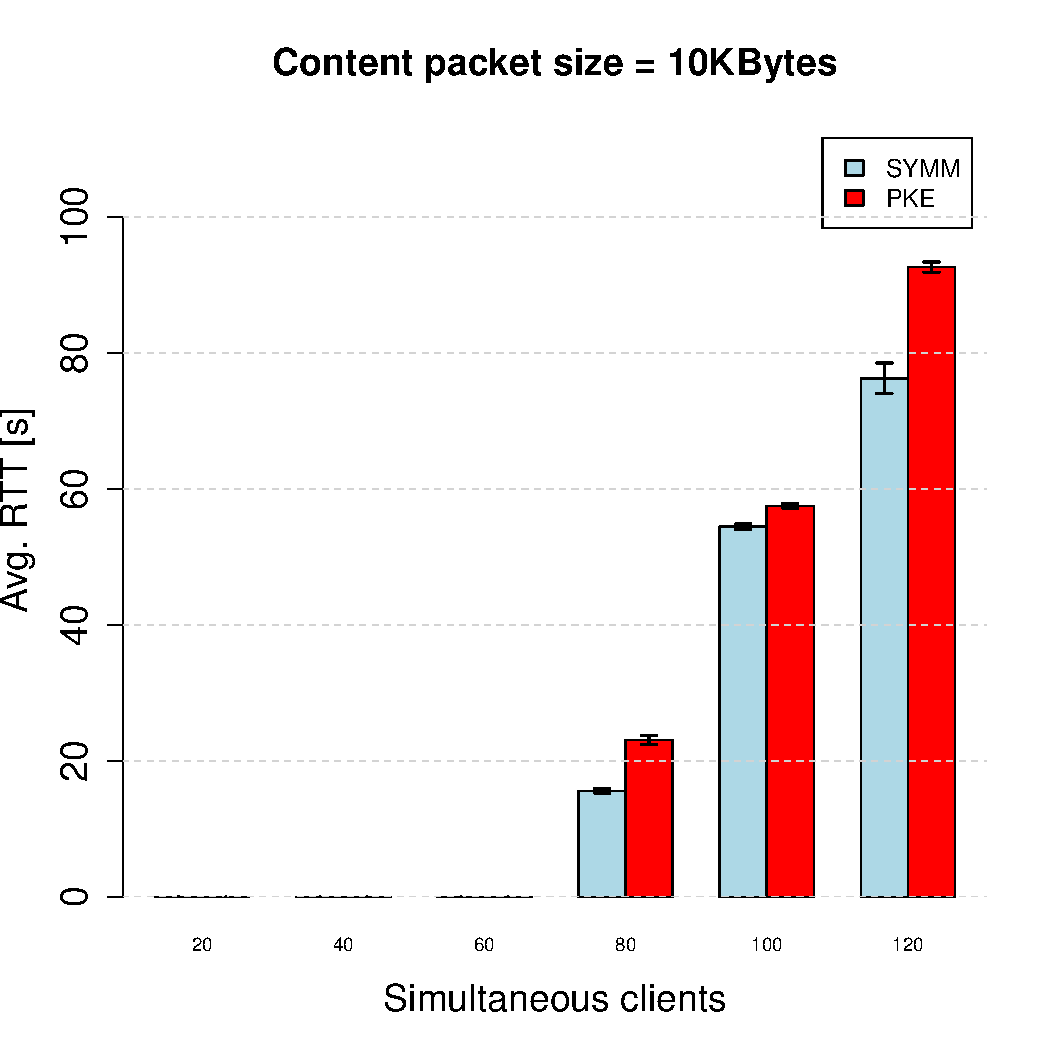
\includegraphics[width=0.8\columnwidth]{images/n_n_rtt.pdf}\label{1b}}
\caption{CCVPN performance with multiple consumers and multiple producers. Each consumer requests with 1 mbps rate.}\label{exp1}
\end{figure}


CCVPN is implemented as a network layer service running on the gateways of the private networks that compose the VPN (see Fig.\ref{fig:ccvpn}).
Our implementation uses the CCNx software stack~\cite{CCNxGithub} and the cryptographic library Sodium~\cite{sodiumGithub}. These are both publicly available and written in C.
For the PKE version of CCVPN, we use Sodium Sealed-Boxes~\cite{bernstein2006curve25519}, implemented over X25519 elliptic curves, as the PKE algorithm for the interest encapsulation and decapsulation routines (Algorithm~\ref{alg:interestEncap}, and Algorithm~\ref{alg:interestDecap} of Sec.~\ref{metho}).
AES256-GCM~\cite{dworkin2007recommendation} is used to encrypt-then-MAC content responses (Alg.~\ref{alg:contentEnc}, and Alg.~\ref{alg:contentDec} of Sec.~\ref{metho}).
Recall that the symmetric keys used to encrypt-then-MAC the content packets are generated and sent together with the encapsulated interest in Alg.~\ref{alg:interestEncap}.
In the symmetric key version of the design, both, interests and contents, are encapsulated using AES256-GCM under the assumption that the gateways already share symmetric key.


The experiments presented throughout this section were executed in an Intel Core i7-3770 octacore CPU @3.40GHz, with 16GB of RAM, running Linux (Ubuntu 14.04LTS). Content payload sizes were set to 10 kilobytes.
On every experiment, each of the two gateway processes (i.e., consumer side gateway process, and producer side gateway process) were assigned as a high priority processes and each of them ran in a single core of the processor.
Fig.~\ref{times} presents boxplots for the execution times of the four algorithms involved in CCVPN's data transmission, including both, PKE and Symm. Key versions for interest encapsulation and decapsulation.

With the goal of evaluating the impact of CCVPN's cryptographic overhead on the overall network performance, we measure the network throughput and the request-response round trip time (RTT) under different topology settings.
In our testbed network, the consumers' side and the producers' side gateways are directly interconnected. $N$ producers are connected to the producers' domain gateway and $M$ consumers are connected to the consumers' domain gateway, as illustrated in Fig.~\ref{testnet}.
Under such topology we consider three variations for the values of ${M,N}$:

\begin{itemize}
 \item \textbf{One consumer and one producer $[1,1]$}:
 \item \textbf{Multiple consumers and one producer $[M,1]$}:
 \item \textbf{Multiple consumers and multiple producers $[M,N]$}:
\end{itemize}

\subsection{Discussion}

\todo{TODO: Add results discussion}

